\documentclass{beamer}
\usetheme{Boadilla}

\title{Using Machine Learning to Predict Airbnb Rental Price in New York City}
%\subtitle{Using Beamer}
\author{Andy Vu}
\institute{University of Trento}
\date{\today}

\begin{document}

\begin{frame}
\titlepage
\end{frame}

\begin{frame}
  \frametitle{Outline}
  \tableofcontents
\end{frame}

\section{A little bit about myself}

\begin{frame}
  \frametitle{A little bit about myself}
  \begin{itemize}
    \item I'm a second year master student in Economics
    \item My background is in finance and banking. I spent 2 years working for a
commercial bank in Vietnam.
    \item Research interest:My interest in applying statistical learning in
      forecasting started when I took a course on econometrics. I worked on a
      project on forecasting the electricity price using time series data. Since
      then, I have focused more on data mining, machine learning, and data
      science. My favorite book is "An Introduction to Statistical Learning" by
      Gareth James, Trevor Hastie. Besides reading, I took some courses on data
      analysis, applied machine learning, and programming.
    \item Technical Skills
      \begin{itemize}
        \item Languages: R, Python, Java, SQL
        \item Version Control: Git, Github
        \item Markup Languages: Markdown, \LaTeX

      \end{itemize}


\end{itemize}

\end{frame}

\section{The Problem}
\begin{frame}
  \frametitle{The Problem}
  Two Big Questions:
  \begin{enumerate}
    \item Which model has the best performance in predicting the Airbnb Rental
      Price in NYC?
    \item Which features are essential in predicting the rental price?
  \end{enumerate}
\end{frame}

\section{The Solution}

\begin{frame}
  \frametitle{The Solution- Machine Learning Approach}
  \begin{figure}
  \centering
  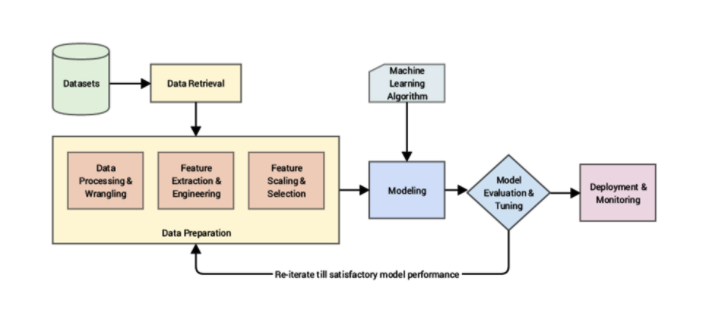
\includegraphics[scale=0.5]{figures/ml-pipeline.png}
  \caption{Machine Learning Pipeline}
  \end{figure}

\end{frame}

\subsection{Airbnb in New York}

\begin{frame}
  \frametitle{Airbnb New York City}

  \begin{figure}
  \centering
  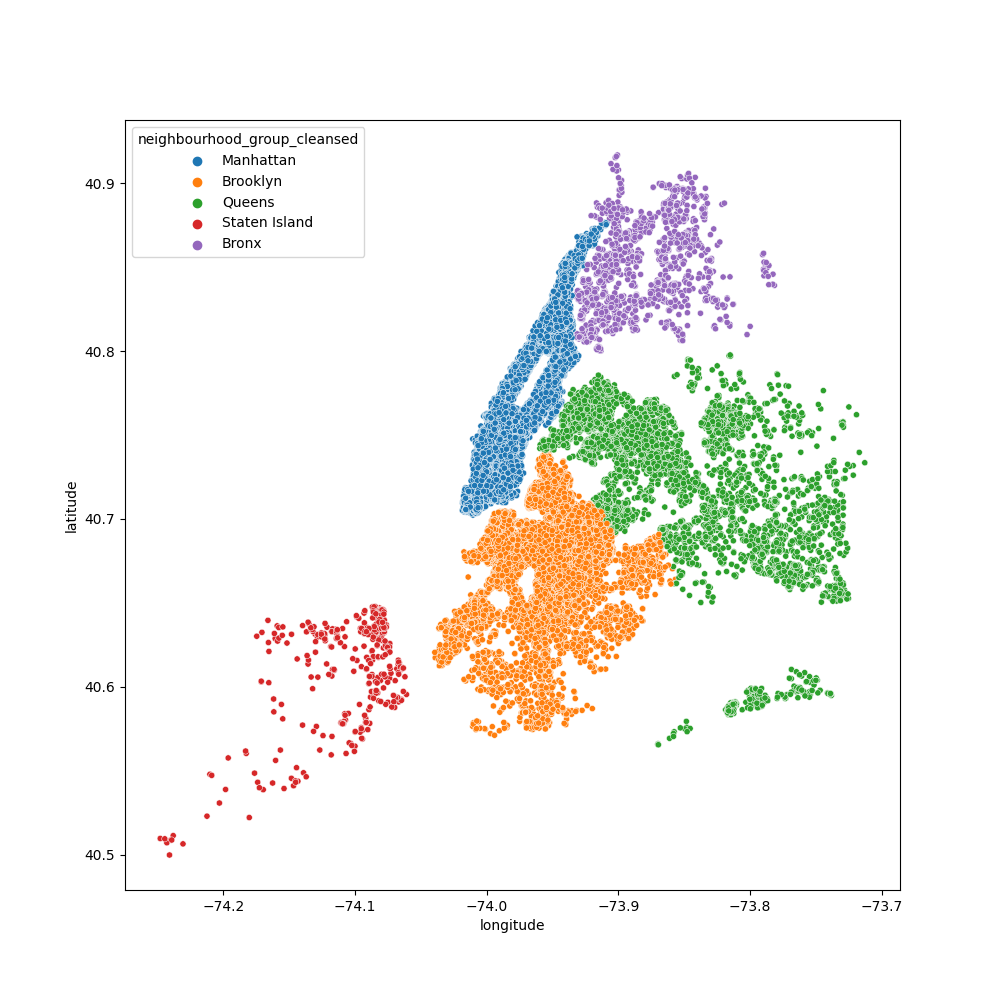
\includegraphics[width=0.7\textwidth]{figures/airbnb-map.png}
\end{figure}

\end{frame}

\subsection{Dataset}

\begin{frame}
  \frametitle{The Dataset}
 \begin{itemize}
    \item Source: The data comes from InsideAirbnb.com, a group that scraped the
      from the Airbnb website.
    \item Data Preprocessing: The data is untidy and not ready for model
      fitting, so we perform data filtering, feature selection, missing value
      handling, feature binning, data transformation.
    \item Features: The final dataset after the preprocessing step has 39907
      observations with 279 features.
  \end{itemize}

A Glimpse of some features:
\begin{flushleft}
\begin{table}[htpb]
    \caption{The variable list}
    \label{tab:variable-list}
    \resizebox{\textwidth}{!}{%
    \begin{tabular}{ll}
    \hline
    Variables & Definition \\
    \hline
    experience\_offerd & recommended category of travel type, e.g. business \\
    host\_since & date that the host first joined Airbnb \\
    host\_response\_time & average amount of time the host takes to reply to messages \\
    host\_response\_rate & proportion of messages that the host replies to \\
    host\_is\_superhost &
    \begin{tabular}{@{}l@{}l@{}} whether or not the host is a superhost, which is a
        mark of \\ mark of quality for the top-rated and most experienced hosts,
        \\ and can increase your search ranking on Airbnb \end{tabular} \\
    host\_listings\_count & how many listings the host has in total \\
\end{tabular}}
\end{table}
\end{flushleft}


\end{frame}

\subsection{Exploratory Data Analysis}

\begin{frame}
  \frametitle{Data Visualization}
  \framesubtitle{Listing capacity}
 A listing's price seems to be positive associated with the number of guests
  it can accommodate.
\begin{figure}[H]
    \centering
        \centering
        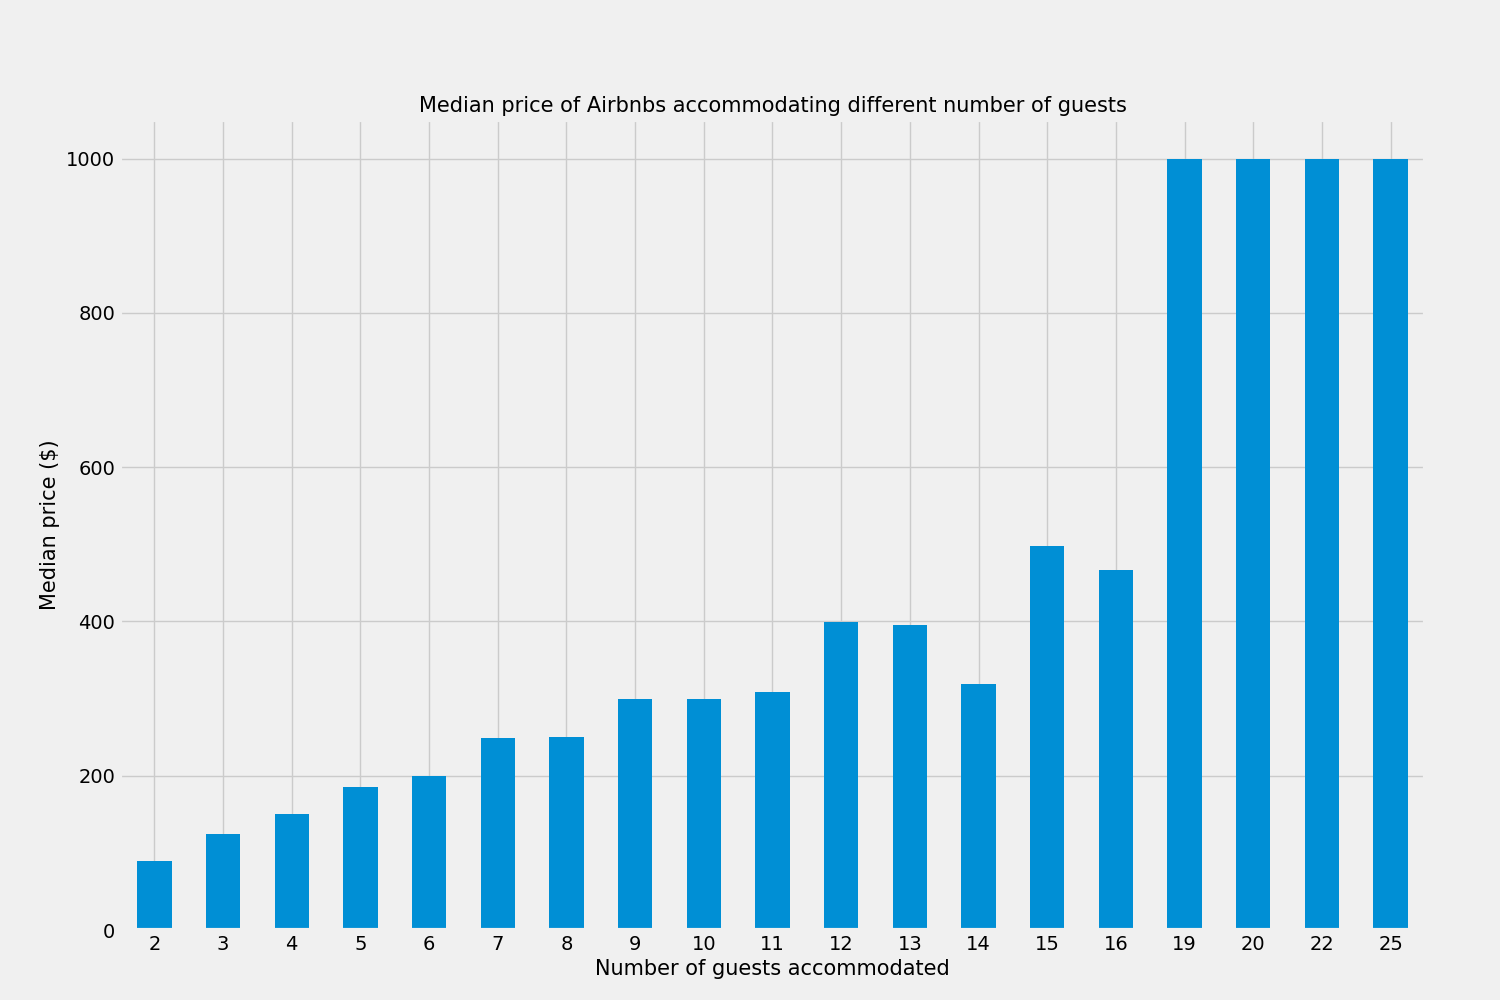
\includegraphics[width=0.7\textwidth]{figures/Figure_8.png}
        \caption{Median Price according to  accomodates}
        \label{fig:median-price-by-accommodates}
      \end{figure}
\end{frame}

\begin{frame}
  \frametitle{Data Visualization}
  \framesubtitle{Location Features}
The location might have an important role in determining the price. Unsurprisingly,
listing in the city center (Manhattan and Brooklyn) has a higher median rental price.
\begin{figure}[H]\centering
  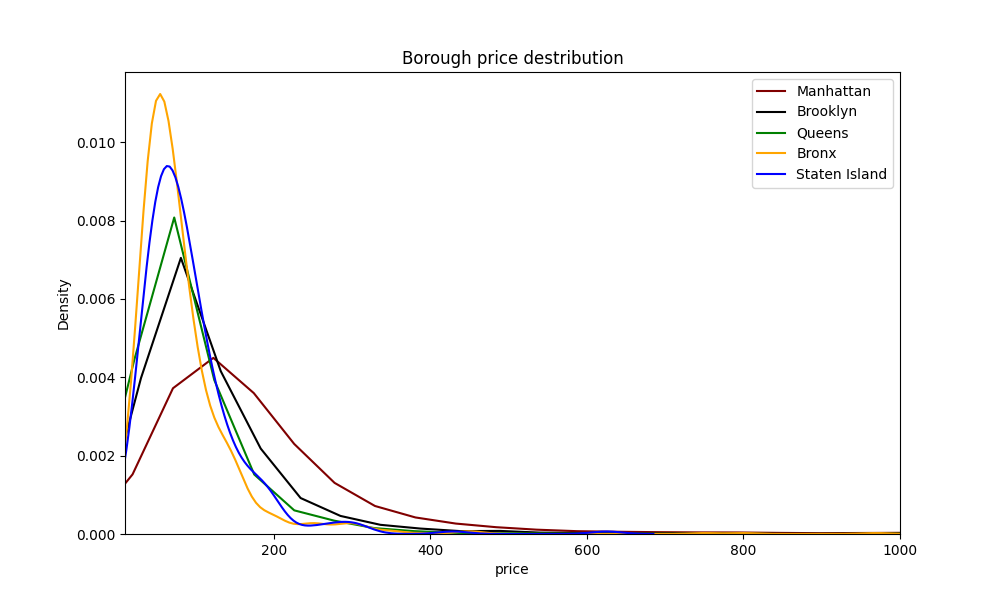
\includegraphics[width=0.7\textwidth]{figures/Figure_11_b.png}
    \caption{Borough Price Distribution}
    \label{fig:borough-price-distribution}
\end{figure}
\end{frame}

\begin{frame}
  \frametitle{Data Visualization}
  \framesubtitle{Superhost status}
  \begin{columns}
    \column{0.5\textwidth}
Hosts with superhost status usually charge higher prices. A possible explanation
for this might be that people are willing to pay a premium price because they
consider superhost status a mark of quality.
\column{0.5\textwidth}
      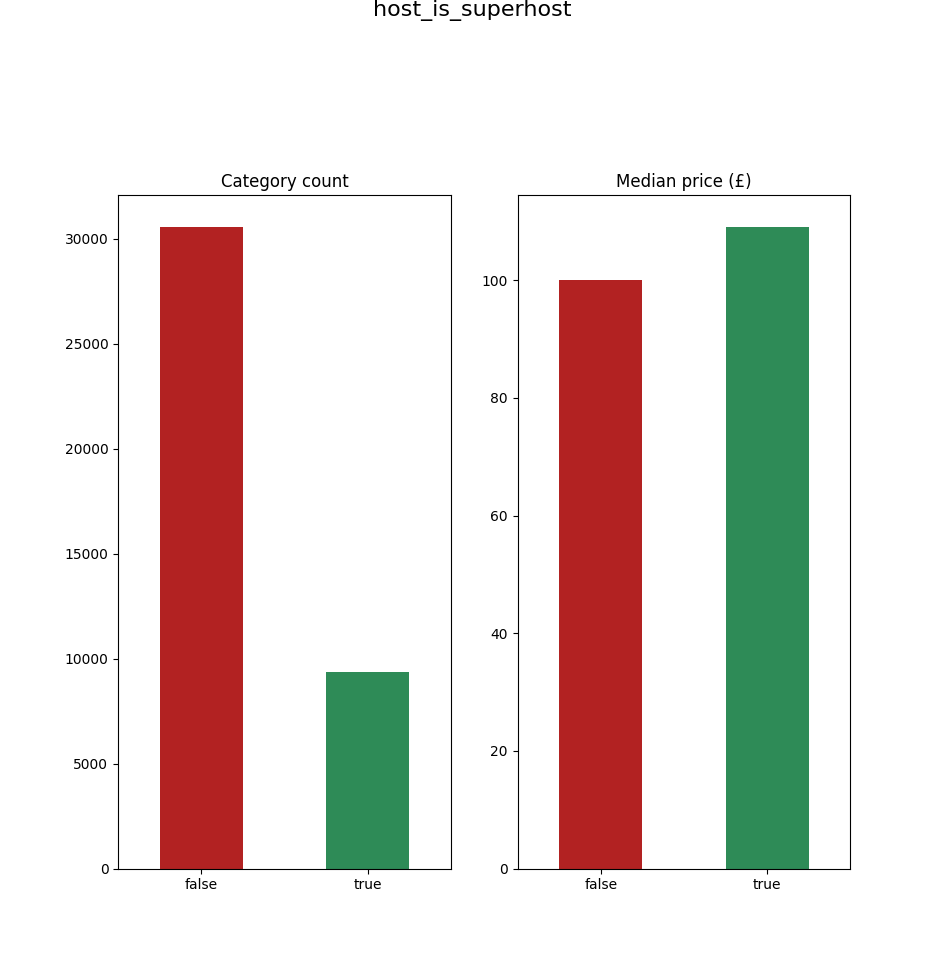
\includegraphics[width=\textwidth]{figures/Figure_16_host_is_superhost.png}
  \end{columns}
\end{frame}


\begin{frame}
  \frametitle{Data Visualization}
  \framesubtitle{Host Verification}
  \begin{columns}
    \column{0.5\textwidth}
Hosts with verified profiles gain a price premium. The relationship may be
explained by the fact that verified profiles (e.g., by providing ID and
verifying your phone number and email address) can increase their
trustworthiness and, therefore, can charge a higher rental price.
  \column{0.5\textwidth}
        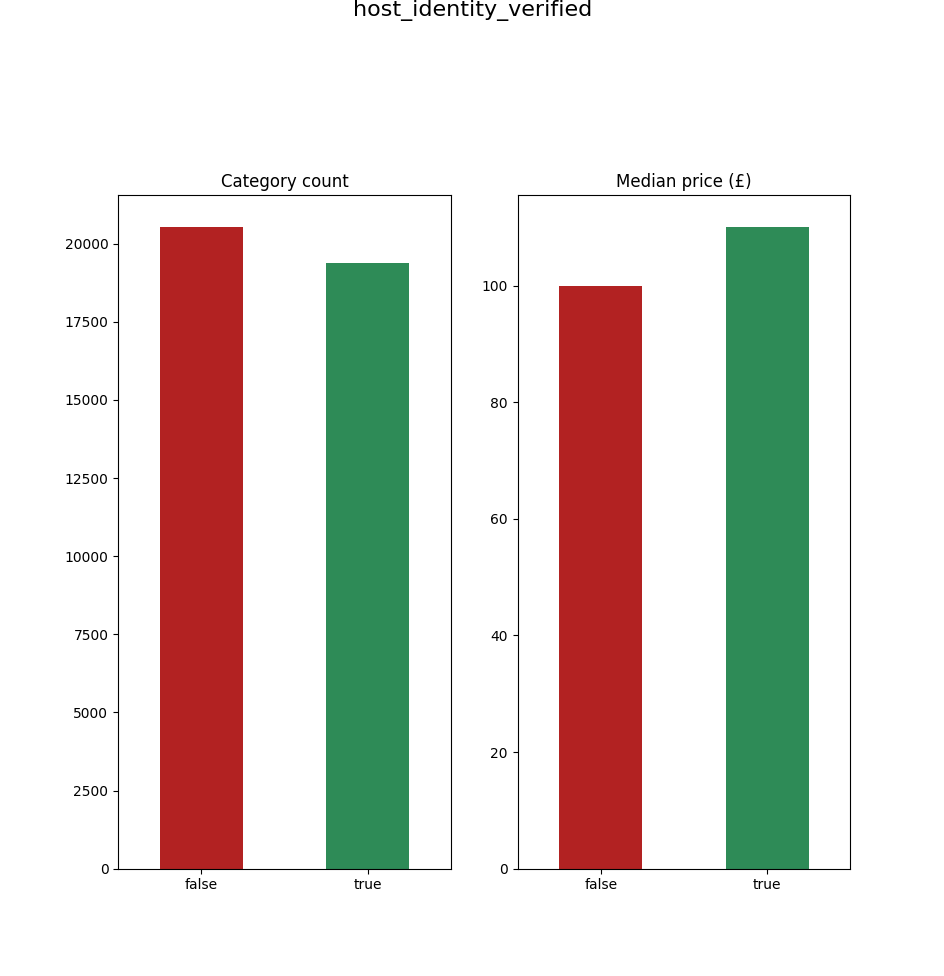
\includegraphics[width=\textwidth]{figures/Figure_16_host_identity_verified.png}
  \end{columns}
\end{frame}

\subsection{Algorithms Used}

\begin{frame}
  \frametitle{How to Assess One Model Performance?}
We can assess how well a model performs by using mean square error criteria
\begin{eqnarray}
    \label{eqn:mse}
    MSE = \frac{1}{n} \sum_{i=1}^{n}(y_i - \hat{f}(x_i))^2
\end{eqnarray}

The best model is the one that has the lowest \textit{test} MSE (not
\textit{training} MSE)
\end{frame}

\begin{frame}
  \frametitle{Variance-Bias Tradeoff}

The expected test MSE, for a given value $x_0$, can be broken down into three
parts as followed:
  \begin{eqnarray}
  E(y_0 - \hat{f}(x_{0}))^2 =  \textrm{Var}(\epsilon) +
  [\textrm{Bias}(\hat{f}(x_{0})]^2 + \textrm{Var}(\hat{f}(x_{0}))
  \label{eqn:variance-bias-tradeoff}
  \end{eqnarray}

\textbf{Comments:}
\begin{itemize}
  \item Minimizing the test MSE means reducing the combination of bias and variance.
  \item However, it is impossible to do both simultaneously. Too simple model
    (low variance) tends to have high bias and too complex model (low bias) is likely to vary significantly.
\end{itemize}
\end{frame}

\subsection{Modelling Strategy}

\begin{frame}
  \frametitle{Modelling Strategy}
We employ some commonly-used algorithms to find the one with the lowest
  \texttt{Test MSE} :
  \begin{enumerate}
    \item Linear Regression with the full number of features - This model is
      expected to be overfitting because it tries to fit a huge number of
      features.
    \item Ridge Regression: An improvement to Linear Regression as it tries to
      overcome overfitting by constraining the coefficient parameters.
    \item Lasso Regression: Similar to Ridge Regression but have an advantage of
      being able to perform \textit{feature selection}.
    \item XGboost: decision-tree-based ensemble Machine Learning algorithm
      that uses a gradient boosting framework.

  \end{enumerate}
\end{frame}



\subsection{Main Findings}

\begin{frame}
  \frametitle{Which model performs the best?}
    \begin{table}[htpb]
      \centering
      %\caption{Results}
      \label{tab:results}

    \resizebox{0.8\textwidth}{!}{%
      \begin{tabular}{lllll}
        \hline
        ML Algorithm & Training MSE & Test MSE & Training $R^2$ & Test $R^2$ \\
        \hline
        Linear Regresion & 0.1291 &  8.5E21 &  0.7019 & -1.9E22 \\
        Ridge Regression  & 0.1291 & 0.138 & 0.7019 &  0.6857 \\
        Lasso Regression & 0.1351 & 0.1441 & 0.688 & 0.6718 \\
        XGboost &  0.0798 & 0.1173 & 0.8157 &  0.7328 \\
    \end{tabular}}
    \end{table}

    Comments:
  \begin{itemize}
      \item As expected, Linear Regression has the worst performance. The
        \texttt{Test MSE} and $R^2$ is very large and much higher than other models.
      \item Ridge and Lasso do much better both in terms of Test MSE and $R^2$.
        While Lasso performance is not as good as Ridge, it has the advantage of
        producing of \textit{sparser} model with just 153 features compared to
        that of 278 features of Ridge.
      \item XGboost has the best performance among all models.
    \end{itemize}
\end{frame}

\begin{frame}
 \frametitle{Which features are essential to predict the rental price?}
\begin{table}[H]
  \centering
  \caption{XGBoost Top 10 Feature Weights}
  \label{tab:xgb-weights}
\resizebox{0.6\textwidth}{!}{%
  \begin{tabular}{lr}
    \toprule
    {} &    weight \\
    \midrule
    room\_type\_Entire home/apt        &  0.336396 \\
    bathrooms                        &  0.032001 \\
    neighbourhood\_Midtown            &  0.025008 \\
    neighbourhood\_Hell's Kitchen     &  0.018545 \\
    neighbourhood\_East Village       &  0.015763 \\
    property\_type\_Other              &  0.015168 \\
    neighbourhood\_Bedford-Stuyvesant &  0.014314 \\
    neighbourhood\_West Village       &  0.014031 \\
    neighbourhood\_Chelsea            &  0.013612 \\
    neighbourhood\_Lower East Side    &  0.011874 \\
  \bottomrule
\end{tabular}}
\end{table}
\end{frame}

\begin{frame}
  \frametitle{Which features are importance in predict the rental price?}
  Comments:
 \begin{itemize}
    \item The most important positive features are whether the type of listing is the
  entire home.
    \item Features related to the location are in the top 10.  Being in  Hell's
    Kitchen, Midtown, East Village, Chelsea, West Village, Upper West Side,
    Williamsburg, Upper East Side, SoHo, Lower East Side neighborhood is associated
    with an increase in the listing price.
  \end{itemize}
\end{frame}

\subsection{Future Works}

\begin{frame}
  \frametitle{Future Works}
  \begin{itemize}
    \item Experiment the data with deep learning algorithms.
    \item Find a way to incorporate customer reviews feature through sentiment
  \end{itemize}

\end{frame}

\subsection{Software Used}

\begin{frame}
  \frametitle{Software Used}

\begin{description}
  \item[Python]: a general-purpose programming language used in many data
    science applications
  \item[Pandas] : a Python library for data wrangling and analysis
  \item[Scikit-learn]: the most promient Python library for machine learning.
  \item[Matplotlib and Seaborn]: the primary plotting libraries in Python
  \item[Other libraries and packages]: geopandas (for plotting geographical
    data), xgboost (for XGboost algorithms)
\end{description}
\end{frame}


\end{document}

